% vim: set wrap

%The first published attempt at writing a program to play Havannah is a BSc thesis by Terry Rogers in 2004. In his thesis, he describes implementing several very weak strategies, easily beaten by a human who was just introduced to the game. An alpha-beta player has been attempted, as shown by Johan de Koning's program PZN, which was blind to rings. The majority of the literature about playing Havannah is based on Monte-Carlo Tree Search though. Monte-carlo Tree Search is well suited to Havannah, as there is no known good heuristic. It also has several similarities to the games of Go and Hex where MCTS has been shown to work very well.

%Several papers have been written about playing Havannah before. Teytaud\cite{teytaud2010creating} showed that UCT and RAVE work well in Havannah. Fossel\cite{fossel2010monte} showed that RAVE works well and tested a few other features. He found that checking for a winning moves (mate-in-one moves) in the rollout improves the playouts and therefore the strength. Lorentz\cite{lorentz2011improving} also tested checking for mate-in-one moves as well as blocking those moves and found an improvement. He used a rollout policy to encourage playing near previous stones. He backed up proven positions within the tree, potentially solving the root board position. He also found success with progressive widening.

These are early days for developing strong Havannah programs. The first published attempt at writing a program to play Havannah is a BSc thesis by Terry Rogers in 2004 \cite{rogers2004bsc}. In his thesis, he describes implementing several weak strategies, easily beaten by even the most amateur human player. The only alpha-beta based Havannah program is Johan de Koning's program PZN, which competed in the 2010 ICGA Olympiad. It finished in last place because its heuristic function, which is quite similar to the distance to win heuristic shown in Section \ref{sec:distwin}, is blind to rings, virtual connections and most threats, and is too slow to for alpha-beta to reach sufficient depths for that to not matter. The majority of attempts, and particularly published attempts, have been Monte-Carlo Tree Search based, primarily because MCTS does not need a heuristic evaluation function. This has also been influenced by MCTS's recent successes in the similar games of Go and Hex where MCTS has overtaken traditional techniques. Given this, MCTS is a good starting point for writing a Havannah player. This chapter will explore the performance of various search algorithms and enhancements as applied to Havannah using the Havannah program named Castro.\footnote{https://github.com/tewalds/castro}

UCT has strong guarantees about eventual optimality, so is the first baseline. After a few games, an exploration constant of 0.9 was chosen as a reasonable value to test against. RAVE has been shown by Teytaud to be strong in Havannah\cite{teytaud2010creating}, and this finding will be confirmed in Section \ref{sec:playingrave}. For all tests thereafter, a RAVE player will be used as the baseline player. The RAVE baseline has no UCT exploration, keeps the tree between moves, and does 2-ply node expansion backups. Unless otherwise stated, all data points are based on several hundred games played with 5 seconds per move.


\section{Testing Methodology}

All testing was done using ParamLog,\footnote{https://github.com/tewalds/ParamLog} an open source distributed testing framework written for this project. Tests were run on board sizes 4 through 10 with 1, 2, 5 and 10 seconds per move. The times are standardized to a machine that can complete 500,000 simulations on size 4 with basic UCT in 11 seconds, which is approximately equal to a Core 2 Duo 2.4ghz. This has the added effect of keeping results comparable across machines and in the face of optimizations. Only the results from the tests with 5 seconds are shown, because this has been common among other published papers about Havannah, but also because most test cases are fairly consistent between different amounts of time.

All tests are played relative to a baseline. The first baseline is UCT.


\section{RAVE}\label{sec:playingrave}

RAVE was introduced in Section \ref{sec:rave} as a way to use the information from rollouts during future descents. Teytaud tested RAVE in Havannah in 2010\cite{teytaud2010creating}, yielding a 100\% winrate against UCT with a small number of simulations. Here we used the RAVE formula \eqref{eqn:rave2}: $$ \beta = \frac{k}{k+n_i.n}$$ and test many values for $k$. Figure \ref{fig:ravegraph} shows the results. $k=500$ yields a greater than 80\% win rate on all board sizes, and so is chosen as the baseline for all future tests. This is equivalent to a 250 or more elo gain.

% To test that $k=500$ is a strong value, we tested different rave values against the rave baseline, with the results shown in Figure \ref{fig:raverave}.

\begin{figure}
	\centering
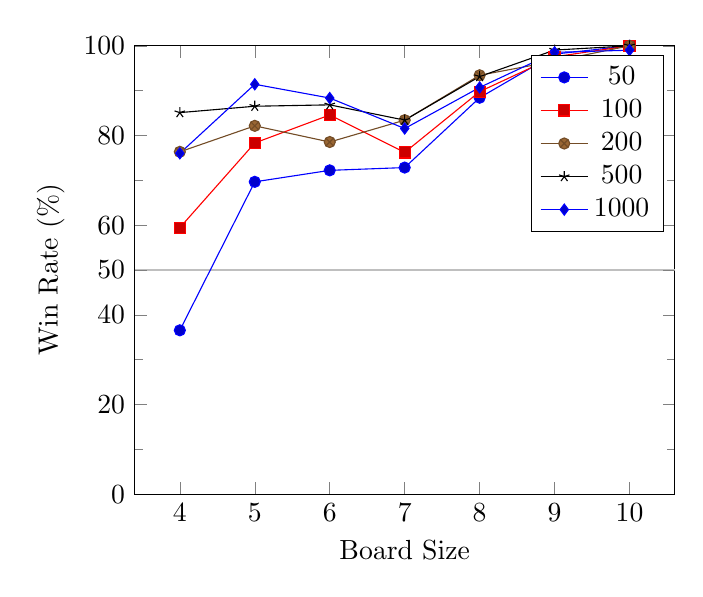
\begin{tikzpicture}
\begin{axis}[
	xlabel=Board Size,
	ylabel=Win Rate (\%),
	xtick={4,5,6,7,8,9,10},
	ymin=0, ymax=100,
	minor y tick num=1,
	extra y ticks={50},
	extra y tick style={grid=major},
]
\addplot coordinates { (4,36.54) (5,69.66) (6,72.22) (7,72.84) (8,88.42) (9,98.15) (10,100.00) }; \addlegendentry{   50}
\addplot coordinates { (4,59.43) (5,78.33) (6,84.57) (7,76.22) (8,89.78) (9,97.55) (10,100.00) }; \addlegendentry{  100}
\addplot coordinates { (4,76.35) (5,82.15) (6,78.54) (7,83.42) (8,93.43) (9,96.58) (10,100.00) }; \addlegendentry{  200}
\addplot coordinates { (4,85.10) (5,86.52) (6,86.83) (7,83.42) (8,93.15) (9,99.05) (10,100.00) }; \addlegendentry{  500}
\addplot coordinates { (4,76.02) (5,91.42) (6,88.35) (7,81.55) (8,90.71) (9,98.54) (10,99.02) }; \addlegendentry{ 1000}
\end{axis}
\end{tikzpicture}
	\caption{Rave vs UCT Baseline}
	\label{fig:ravegraph}
\end{figure}

%\begin{figure}
%	\centering
%\begin{tikzpicture}
%\begin{axis}[
%	xlabel=Board Size,
%	ylabel=Win Rate (\%),
%	xtick={4,5,6,7,8,9,10},
%	ymin=0, ymax=100,
%	minor y tick num=1,
%	extra y ticks={50},
%	extra y tick style={grid=major},
%]
%%\addplot coordinates { (4,22.47) (5,19.33) (6,27.58) (7,20.11) (8,15.32) (9,19.62) (10,25.48) }; \addlegendentry{   20}
%%\addplot coordinates { (4,47.78) (5,45.57) (6,40.97) (7,28.53) (8,32.44) (9,38.61) (10,45.98) }; \addlegendentry{   50}
%\addplot coordinates { (4,47.57) (5,44.35) (6,54.83) (7,42.93) (8,46.54) (9,51.54) (10,56.27) }; \addlegendentry{  100}
%\addplot coordinates { (4,46.09) (5,52.01) (6,58.26) (7,45.40) (8,50.61) (9,49.38) (10,56.55) }; \addlegendentry{  200}
%\addplot coordinates { (4,49.00) (5,53.32) (6,51.26) (7,51.25) (8,50.14) (9,48.68) (10,50.10) }; \addlegendentry{  500}
%\addplot coordinates { (4,55.87) (5,58.10) (6,50.84) (7,37.24) (8,49.18) (9,41.07) (10,34.17) }; \addlegendentry{ 1000}
%%\addplot coordinates { (4,59.47) (5,51.04) (6,47.59) (7,40.70) (8,41.63) (9,38.84) (10,36.29) }; \addlegendentry{ 1500}
%%\addplot coordinates { (4,51.24) (5,42.30) (6,37.13) (7,38.49) (8,46.54) (9,38.74) (10,33.47) }; \addlegendentry{ 2000}
%%\addplot coordinates { (4,54.81) (5,37.45) (6,33.75) (7,31.93) (8,50.00) (9,39.62) (10,32.56) }; \addlegendentry{ 5000}
%%\addplot coordinates { (4,43.30) (5,30.93) (6,29.50) (7,35.50) (8,47.54) (9,38.04) (10,38.79) }; \addlegendentry{10000}
%\end{axis}
%\end{tikzpicture}
%	\caption{Rave vs Rave baseline}
%	\label{fig:raverave}
%\end{figure}


\section{Keep Tree Between Moves}

MCTS builds a large tree with real experience, and then makes a move. Most of the final move selection strategies will choose a large subtree usually consisting of more than 25\% of the effort that went into this move choice, but often consisting of as much as 95\% of the work. This is real experience that would be duplicated after the next move if it was thrown away. The opponent's move is unknown at this point, but is frequently the expected reply, again often maintaining 25\% or more of the tree. Keeping the remaining tree is a pure advantage with no downsides. Keeping the the tree has about a 53\% winning rate against throwing away the tree after each move. This is not a huge improvement, but is easy, free and works on all board sizes.

%\begin{figure}
%\centering
%\begin{tikzpicture}
%\begin{axis}[
%	xlabel=Board Size,
%	ylabel=Win Rate (\%),
%	xtick={4,5,6,7,8,9,10},
%	ymin=0, ymax=100,
%	minor y tick num=1,
%	extra y ticks={50},
%	extra y tick style={grid=major},
%]
%\addplot coordinates { (4,47.57) (5,46.55) (6,45.49) (7,49.35) (8,47.48) (9,46.58) (10,46.60) }; \addlegendentry{Disabled}
%\end{axis}
%\end{tikzpicture}
%	\caption{Disable Keep Tree vs RAVE baseline}
%	\label{fig:keeptree}
%\end{figure}


\section{Proof Backups}\label{sec:proofbackups}

\begin{figure}
	\centering
	\begin{HavannahBoard}[board size=4,coordinate style=classical,show coordinates=false]
%	\HGame{b1,d2,a2,e4}
	\HStoneGroup[color=white]{b1,a2}
	\HStoneGroup[color=black]{d2,e4}
	\end{HavannahBoard}
	\caption{Early Position Solvable by MCTS in 1 Minute, white to play}
	\label{fig:lorentzproof}
\end{figure}

\begin{figure}
\centering
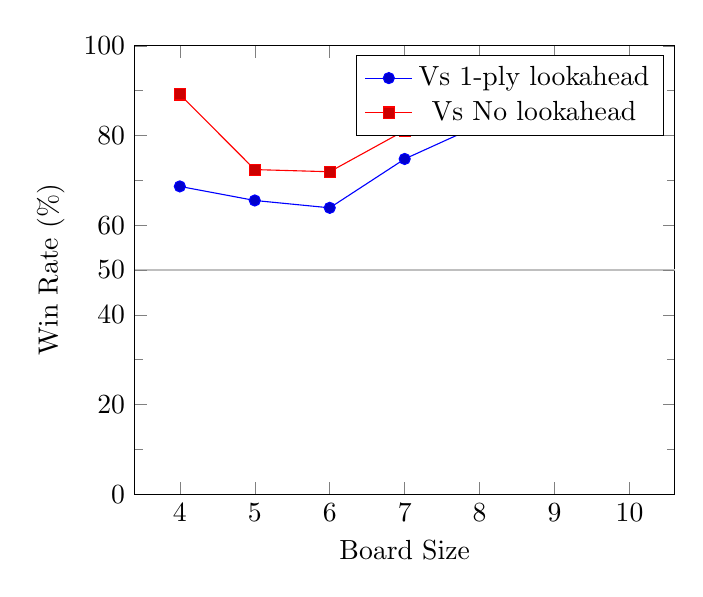
\begin{tikzpicture}
\begin{axis}[
	xlabel=Board Size,
	ylabel=Win Rate (\%),
	xtick={4,5,6,7,8,9,10},
	ymin=0, ymax=100,
	minor y tick num=1,
	extra y ticks={50},
	extra y tick style={grid=major},
]
\addplot coordinates { (4,68.64) (5,65.5) (6,63.86) (7,74.76) (8,82.35) (9,84.24) (10,84.88) }; \addlegendentry{Vs 1-ply lookahead}
\addplot coordinates { (4,89.15) (5,72.39) (6,71.91) (7,81.1) (8,86.63) (9,84.99) (10,87.32) }; \addlegendentry{Vs No lookahead}

%\addplot coordinates { (4,31.36) (5,34.50) (6,36.14) (7,25.24) (8,17.65) (9,15.76) (10,15.12) }; \addlegendentry{One ply}
%\addplot coordinates { (4,10.85) (5,27.61) (6,28.09) (7,18.90) (8,13.37) (9,15.01) (10,12.68) }; \addlegendentry{Disabled}
\end{axis}
\end{tikzpicture}
	\caption{RAVE Baseline with 2-ply lookahead during expansion vs 1-ply lookahead and no lookahead}
	\label{fig:proofbackups}
\end{figure}

A game of Havannah ends when one of the winning conditions is met. This can happen with only a few stones on the board or with the board full of stones. In practice, the game rarely finishes with only a few stones, but frequently the tree includes positions where one player fails to respond correctly to a threat, leading the other player to win easily. MCTS is guided away from allowing these threats as the winning rate drops. By default it will continue trying this losing move as long as it looks better than the others, which could take quite a while. Late in the game, the game tree may be sufficiently small that the entire tree could be enumerated, but normal MCTS will take a long time to converge on the best move. If terminal nodes are marked, and winning moves are backed up as losing moves for their parents and sets of losing moves are backed up as winning moves for their parents, full proof trees can be constructed, allowing faster detection of threats, and proving the outcome of moves late in the game. This has been suggested before, and was explored by Lorentz in 2010 with moderate success \cite{lorentz2011improving}.

Terminal nodes are found in the expansion phase. If a winning move is found, the expansion stops and the parent node is marked as a win. If no winning moves are found, then threats that must be blocked are looked for. If the opponent has exactly one immediate threat, it must be blocked, so all other moves are discarded, and the simulation is continued, expanding that move's children. If the opponent has two or more immediate threats, only one could be blocked, and so the expansion is stopped and the parent is marked as a loss. These outcomes are then propagated as far up the tree as possible.

Lorentz showed a board position, shown here in Figure \ref{fig:lorentzproof}, which his program, Wanderer, solves in 45 minutes. Using RAVE and proof backups but a purely random rollout policy and no heuristic knowledge, Castro solves it in under a minute.

Figure \ref{fig:proofbackups} shows the results from using proof backups. It compares using 2-ply versus 1-ply and 0-ply lookahead. One ply means only checking for winning moves but not checking for the opponent's threats. Two ply means checking for winning moves and for the opponent's threats. Backing up proofs seems to be give a 75-90\% winning rate on all board sizes, which is worth about 100-300 elo. At the olympiad, Castro solved the outcome of the game about 15 moves before the end. Because it keeps the tree between moves, the remaining moves were played out of its precomputed proof tree.


\section{Multiple Rollouts}

Profiling was used to determine where Castro spends its time. Table \ref{tab:phasetime} shows how time is used given 10 seconds to play on an empty board, on board sizes 5 and 10. When using UCT without RAVE, the most of time is spent in rollouts, followed by descent. Expansion and back-propagation, by contrast, take a relatively small amount of time. When using RAVE without exploration, descent takes the most time, with back propagation and rollouts taking most of the rest. Compared to using UCT, RAVE spends less time in rollouts, and more time in descent and back-propagation. While the optimal ratio of time is unknown, spending time evaluating nodes intuitively seems to be a better use of time than the bookkeeping associated with figuring out which nodes to evaluate. To alleviate this, multiple rollouts were run per simulation. This would lower the number of full simulations, but increase the number of rollouts. Given that rollouts are used to approximate the value of a given node, this should increase the accuracy of the experience in the tree, and hopefully the playing strength.


The experience from the rollouts are aggregated before the back-propagation phase so only a single update is needed for the RAVE and experience values of each node in the tree. Figure \ref{fig:multirollouts} shows the results when doing multiple rollouts per simulation, given the same amount of time. Multiple rollouts only has a small benefit on size 4, but is worth 50-100 elo on sizes 5 and up. Two rollouts has a mean winning rate of 55\%, while 15 rollouts has a mean winning rate of 63\%. For comparison, Tables \ref{tab:phasetime2} and \ref{tab:phasetime10} show the time used for 2 rollouts per simulation and 10 rollouts per simulation respectively. Doing 2 rollouts per simulation drops the number of simulations to two thirds, and doing 10 rollouts per simulation drops it to a fifth to a third as many simulations. This is a big drop in simulations, but the total number of rollouts increased more than enough to compensate. This has the added benefit of building a smaller, more accurate tree, reducing memory usage.

\begin{figure}
	\centering
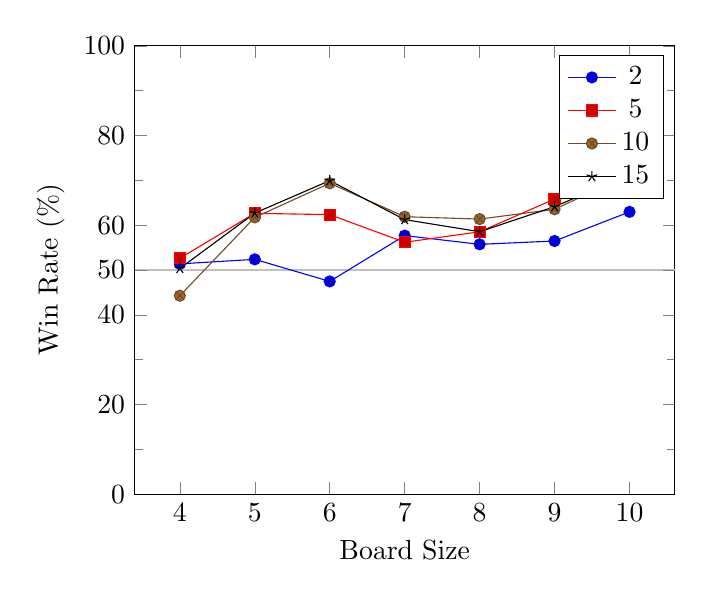
\begin{tikzpicture}
\begin{axis}[
	xlabel=Board Size,
	ylabel=Win Rate (\%),
	xtick={4,5,6,7,8,9,10},
	ymin=0, ymax=100,
	minor y tick num=1,
	extra y ticks={50},
	extra y tick style={grid=major},
]
\addplot coordinates { (4,51.36) (5,52.37) (6,47.45) (7,57.67) (8,55.72) (9,56.46) (10,62.96) }; \addlegendentry{ 2}
%\addplot coordinates { (4,50.62) (5,60.59) (6,54.13) (7,53.38) (8,58.92) (9,58.04) (10,65.88) }; \addlegendentry{ 3}
%\addplot coordinates { (4,51.19) (5,57.16) (6,55.11) (7,56.79) (8,59.25) (9,60.49) (10,70.09) }; \addlegendentry{ 4}
\addplot coordinates { (4,52.61) (5,62.64) (6,62.34) (7,56.18) (8,58.51) (9,65.82) (10,67.59) }; \addlegendentry{ 5}
%\addplot coordinates { (4,49.77) (5,55.93) (6,60.85) (7,56.40) (8,60.65) (9,59.08) (10,73.29) }; \addlegendentry{ 6}
%\addplot coordinates { (4,49.94) (5,59.04) (6,54.70) (7,52.52) (8,57.14) (9,66.13) (10,68.75) }; \addlegendentry{ 7}
%\addplot coordinates { (4,53.40) (5,59.93) (6,67.23) (7,55.61) (8,60.16) (9,68.39) (10,71.20) }; \addlegendentry{ 8}
%\addplot coordinates { (4,49.89) (5,62.83) (6,53.83) (7,59.96) (8,58.12) (9,68.94) (10,70.44) }; \addlegendentry{ 9}
\addplot coordinates { (4,44.26) (5,61.73) (6,69.34) (7,61.88) (8,61.35) (9,63.53) (10,71.33) }; \addlegendentry{10}
%\addplot coordinates { (4,48.01) (5,68.65) (6,66.78) (7,54.74) (8,61.71) (9,63.70) (10,68.99) }; \addlegendentry{12}
\addplot coordinates { (4,50.34) (5,62.69) (6,69.93) (7,61.23) (8,58.53) (9,64.12) (10,71.31) }; \addlegendentry{15}
%\addplot coordinates { (4,47.67) (5,64.08) (6,56.59) (7,53.61) (8,62.60) (9,67.85) (10,77.37) }; \addlegendentry{20}
\end{axis}
\end{tikzpicture}
	\caption[Multiple Rollouts]{Multiple Rollouts per Simulation Against Baseline RAVE Player}
	\label{fig:multirollouts}
\end{figure}

\begin{table}
	\centering
	\begin{tabular}{l|rrrrr}
		             & Iterations & Descent & Expansion & Rollout & Back-propagation \\ \hline
		UCT size 5   & 296136 & 33.6\% & 12.0\% & 48.4\% &  5.9\% \\
		UCT size 10  & 102192 & 24.8\% & 11.3\% & 62.0\% &  2.0\% \\
		RAVE size 5  & 148713 & 45.1\% &  7.3\% & 22.2\% & 25.4\% \\
		RAVE size 10 &  41713 & 42.9\% &  4.8\% & 24.3\% & 28.0\% \\
	\end{tabular}
	\caption{Time Used by MCTS Phase with 1 Rollout per Simulation}
	\label{tab:phasetime}
\end{table}

\begin{table}
	\centering
	\begin{tabular}{l|rrrrr}
		             & Iterations & Descent & Expansion & Rollout & Back-propagation \\ \hline
		UCT size 5   & 201408 & 22.9\% & 7.0\% & 66.1\% &  4.0\% \\
		UCT size 10  &  66945 & 16.3\% & 3.5\% & 78.9\% &  1.3\% \\
		RAVE size 5  & 115704 & 34.7\% & 6.0\% & 32.6\% & 26.6\% \\
		RAVE size 10 &  31962 & 29.4\% & 4.0\% & 37.1\% & 29.6\% \\
	\end{tabular}
	\caption{Time Used by MCTS Phase Using 2 Rollouts per Simulation}
	\label{tab:phasetime2}
\end{table}

\begin{table}
	\centering
	\begin{tabular}{l|rrrrr}
		             & Iterations & Descent & Expansion & Rollout & Back-propagation \\ \hline
		UCT size 5   & 58786 &  6.5\% & 1.4\% & 91.0\% &  1.1\% \\
		UCT size 10  & 16616 &  3.9\% & 0.4\% & 95.4\% &  0.3\% \\
		RAVE size 5  & 49131 & 14.8\% & 3.4\% & 65.6\% & 16.2\% \\
		RAVE size 10 & 12232 & 10.7\% & 1.9\% & 71.1\% & 16.3\% \\
	\end{tabular}
	\caption{Time Used by MCTS Phase Using 10 Rollouts per Simulation}
	\label{tab:phasetime10}
\end{table}


\section{Heuristic Knowledge}\label{sec:knowledge}

Heuristic knowledge was described in section \ref{sec:heuristicknowledge} as a way to bias the descent policy towards moves that are likely to be good before any experience has been gained. Castro implements an extra additive knowledge term using the formula: $$\frac{n_i.k}{\sqrt{n_i.n}}$$ This gives a boost to the node that is independent of the exploration bonus from UCT and independent of the $\beta$ value for RAVE. Each heuristic has some small value, which is multiplied by a tuning constant. The different heuristic values are summed for the final knowledge value for that move.


\subsection{Maintain Virtual Connections}

Virtual connections (VC), as shown in Figure \ref{fig:simplevc}, are a fast way of ensuring two groups can connect or that a group can connect to a remote part of the board. However, this is only true if they are maintained. If the opponent places a piece in one of the two empty cells, a response of playing in the other cell is usually a good move. Thus, a bonus should be given to maintaining these virtual connections.

Figure \ref{fig:maintainvc} shows the results of adding a knowledge bonus of 5, 10, 25, 50 or 100 for maintaining the VC. It seems to work very well on a few sizes with a winning rate as high as 70\%, but in general it does not have a big effect on the larger board sizes. This may be because RAVE inherently finds these moves fairly quickly anyway, or because it focuses more on rings on the larger board sizes, in which case VCs aren't very important.

\begin{figure}
	\centering
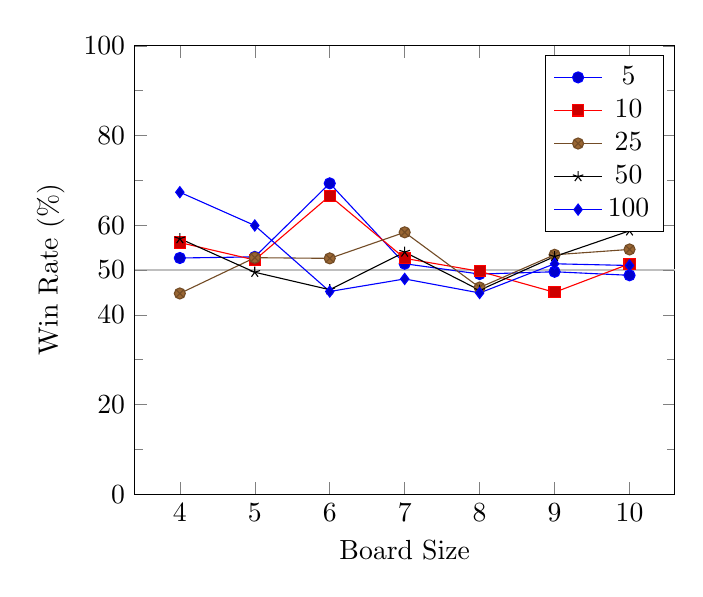
\begin{tikzpicture}
\begin{axis}[
	xlabel=Board Size,
	ylabel=Win Rate (\%),
	xtick={4,5,6,7,8,9,10},
	ymin=0, ymax=100,
	minor y tick num=1,
	extra y ticks={50},
	extra y tick style={grid=major},
]
\addplot coordinates { (4,52.67) (5,52.92) (6,69.32) (7,51.39) (8,49.09) (9,49.60) (10,48.81) }; \addlegendentry{  5}
\addplot coordinates { (4,56.12) (5,52.23) (6,66.53) (7,52.59) (8,49.70) (9,45.02) (10,51.37) }; \addlegendentry{ 10}
\addplot coordinates { (4,44.76) (5,52.74) (6,52.59) (7,58.40) (8,46.09) (9,53.39) (10,54.58) }; \addlegendentry{ 25}
\addplot coordinates { (4,56.99) (5,49.49) (6,45.60) (7,54.00) (8,45.49) (9,52.99) (10,58.73) }; \addlegendentry{ 50}
\addplot coordinates { (4,67.34) (5,59.92) (6,45.20) (7,48.00) (8,44.87) (9,51.38) (10,51.00) }; \addlegendentry{100}
\end{axis}
\end{tikzpicture}
	\caption[Maintain Virtual Connection Bonus]{Maintain Virtual Connection Bonus Against Baseline RAVE Player}
	\label{fig:maintainvc}
\end{figure}



\subsection{Locality}


Large parts of the board are often empty and far from any existing stone, and playing there is rarely a good move. Giving a bonus to positions near existing stones is an intuitively good heuristic. We tested giving a bonus to being near any stone, and also to being near stones of your own colour. The bonus drops off with distance, with a bonus of 3 for a direct neighbour, 2 for forming a VC with an existing stone, and 1 for being distance 2 but not forming a VC. An example of the bonuses around a newly placed stone are shown in Figure \ref{fig:localitypoints}.


\begin{figure}
	\centering
	\begin{HavannahBoard}[board size=3,coordinate style=classical,show coordinates=false]
	\HStoneGroup[color=white]{b2}
	\HStoneGroup[color=light gray,label=3]{a1,a2,b1,c2,c3,b3}
	\HStoneGroup[color=light gray,label=2]{c1,a3,d3,c4}
	\HStoneGroup[color=light gray,label=1]{d2,d4,b4}
	\end{HavannahBoard}
	\caption{Points Given by Distance From an Existing Stone}
	\label{fig:localitypoints}
\end{figure}


First, giving a bonus to being near any stone regardless of colour was tested. The results are shown in Figure \ref{fig:localityany}. While it seemed to help a little bit on bigger boards, in general it was not helpful.

\begin{figure}
	\centering
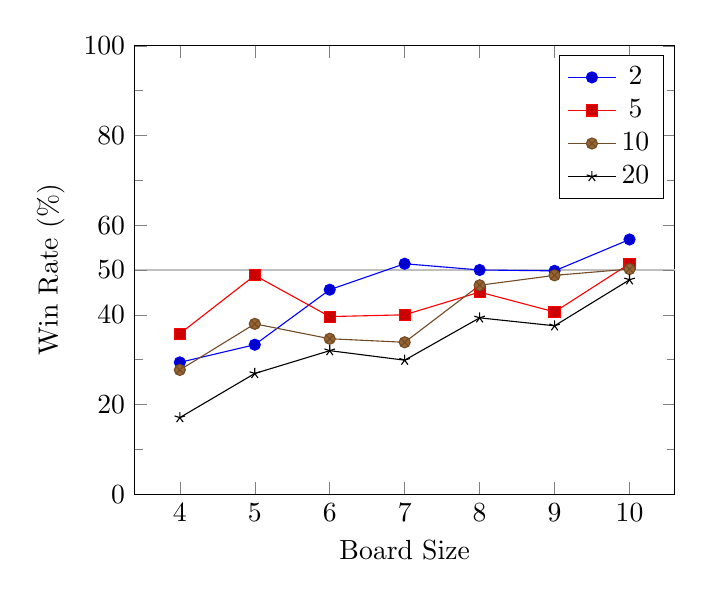
\begin{tikzpicture}
\begin{axis}[
	xlabel=Board Size,
	ylabel=Win Rate (\%),
	xtick={4,5,6,7,8,9,10},
	ymin=0, ymax=100,
	minor y tick num=1,
	extra y ticks={50},
	extra y tick style={grid=major},
]
%\addplot coordinates { (4,40.86) (5,37.30) (6,34.00) (7,48.06) (8,57.03) (9,49.00) (10,42.74) }; \addlegendentry{ 1}
\addplot coordinates { (4,29.39) (5,33.33) (6,45.60) (7,51.39) (8,50.00) (9,49.80) (10,56.80) }; \addlegendentry{ 2}
\addplot coordinates { (4,35.79) (5,48.79) (6,39.60) (7,40.00) (8,45.07) (9,40.64) (10,51.39) }; \addlegendentry{ 5}
\addplot coordinates { (4,27.70) (5,37.98) (6,34.66) (7,33.87) (8,46.59) (9,48.80) (10,50.20) }; \addlegendentry{10}
\addplot coordinates { (4,17.07) (5,26.91) (6,32.00) (7,29.88) (8,39.32) (9,37.55) (10,47.81) }; \addlegendentry{20}
%\addplot coordinates { (4,1.21) (5,18.88) (6,26.98) (7,39.04) (8,31.53) (9,31.47) (10,35.46) }; \addlegendentry{50}
\end{axis}
\end{tikzpicture}
	\caption[Locality Bonus, Any Stones]{Locality Bonus for Playing Near Existing Stones of any Colour Against Baseline RAVE Player}
	\label{fig:localityany}
\end{figure}

Next, giving a bonus for playing near stones of your own colour was tested, as this has been shown to work before \cite{lorentz2011improving, stankiewicz2011knowledge}. The results are shown in Figure \ref{fig:localitysides}, which is much more encouraging. A value of 10 gives a winning ratio of 65\%, or about 100 elo on most board sizes.

\begin{figure}
	\centering
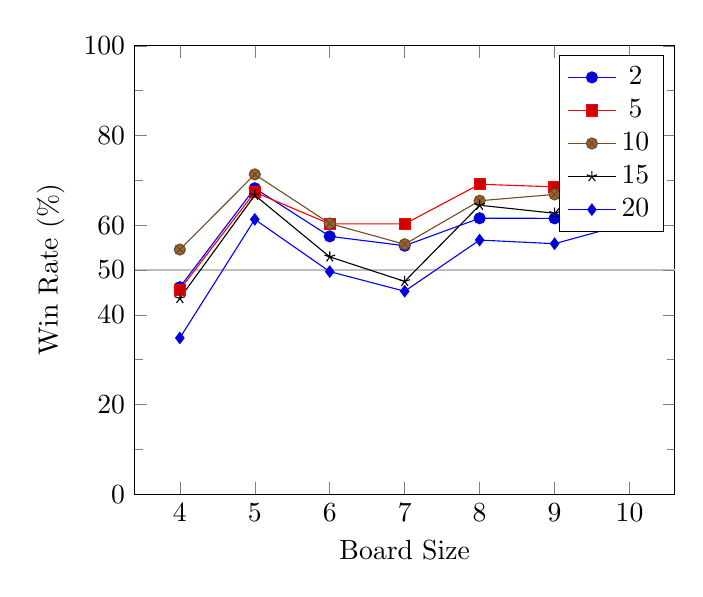
\begin{tikzpicture}
\begin{axis}[
	xlabel=Board Size,
	ylabel=Win Rate (\%),
	xtick={4,5,6,7,8,9,10},
	ymin=0, ymax=100,
	minor y tick num=1,
	extra y ticks={50},
	extra y tick style={grid=major},
]
%\addplot coordinates { (4,55.41) (5,60.06) (6,57.34) (7,46.53) (8,57.76) (9,57.96) (10,61.31) }; \addlegendentry{ 1}
\addplot coordinates { (4,46.15) (5,68.22) (6,57.50) (7,55.41) (8,61.54) (9,61.52) (10,67.02) }; \addlegendentry{ 2}
\addplot coordinates { (4,45.61) (5,67.35) (6,60.27) (7,60.27) (8,69.12) (9,68.54) (10,71.01) }; \addlegendentry{ 5}
\addplot coordinates { (4,54.56) (5,71.32) (6,60.36) (7,55.73) (8,65.44) (9,66.85) (10,76.57) }; \addlegendentry{10}
\addplot coordinates { (4,43.67) (5,66.67) (6,52.92) (7,47.45) (8,64.44) (9,62.65) (10,79.73) }; \addlegendentry{15}
\addplot coordinates { (4,34.83) (5,61.28) (6,49.63) (7,45.26) (8,56.67) (9,55.86) (10,60.44) }; \addlegendentry{20}
%\addplot coordinates { (4,20.90) (5,53.53) (6,43.90) (7,45.20) (8,42.18) (9,47.95) (10,60.00) }; \addlegendentry{50}
\end{axis}
\end{tikzpicture}
	\caption[Locality Bonus, Own Stones]{Locality Bonus for Playing Near Stones of the Same Colour Against Baseline RAVE Player}
	\label{fig:localitysides}
\end{figure}


\subsection{Local Reply}

\begin{figure}
	\centering
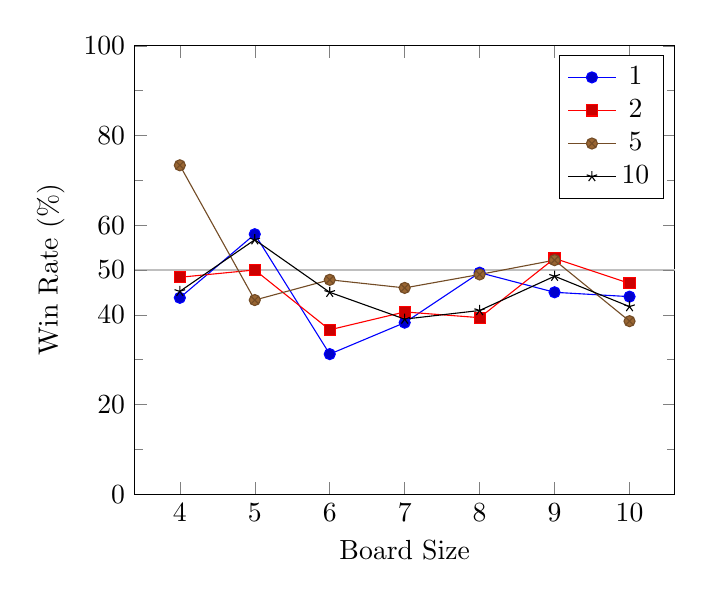
\begin{tikzpicture}
\begin{axis}[
	xlabel=Board Size,
	ylabel=Win Rate (\%),
	xtick={4,5,6,7,8,9,10},
	ymin=0, ymax=100,
	minor y tick num=1,
	extra y ticks={50},
	extra y tick style={grid=major},
]
\addplot coordinates { (4,43.79) (5,57.98) (6,31.23) (7,38.25) (8,49.40) (9,45.02) (10,44.05) }; \addlegendentry{ 1}
\addplot coordinates { (4,48.37) (5,50.00) (6,36.65) (7,40.64) (8,39.36) (9,52.59) (10,47.01) }; \addlegendentry{ 2}
\addplot coordinates { (4,73.35) (5,43.29) (6,47.81) (7,46.00) (8,49.00) (9,52.19) (10,38.58) }; \addlegendentry{ 5}
\addplot coordinates { (4,45.23) (5,56.74) (6,45.02) (7,39.04) (8,40.96) (9,48.61) (10,41.83) }; \addlegendentry{10}
%\addplot coordinates { (4,37.25) (5,31.99) (6,41.20) (7,46.40) (8,38.52) (9,46.83) (10,44.22) }; \addlegendentry{20}
%\addplot coordinates { (4,19.55) (5,27.31) (6,33.33) (7,30.80) (8,19.24) (9,25.69) (10,23.92) }; \addlegendentry{50}
\end{axis}
\end{tikzpicture}
	\caption[Local Reply Bonus]{Local Reply Bonus for Playing Near the Opponent's Last Move Against Baseline RAVE Player}
	\label{fig:localreply}
\end{figure}

Playing well in Havannah often means making defensive moves, replying to the opponent's last move. A bonus is given based on the distance to the opponent's last move. Direct neighbours get a bonus of 3, moves two away get a bonus of 2, and moves three away get a bonus of 1.

The results are shown in Figure \ref{fig:localreply}, showing this heuristic to be not very helpful except on board size 4.



\subsection{Edge Connectivity}

\begin{figure}
	\centering
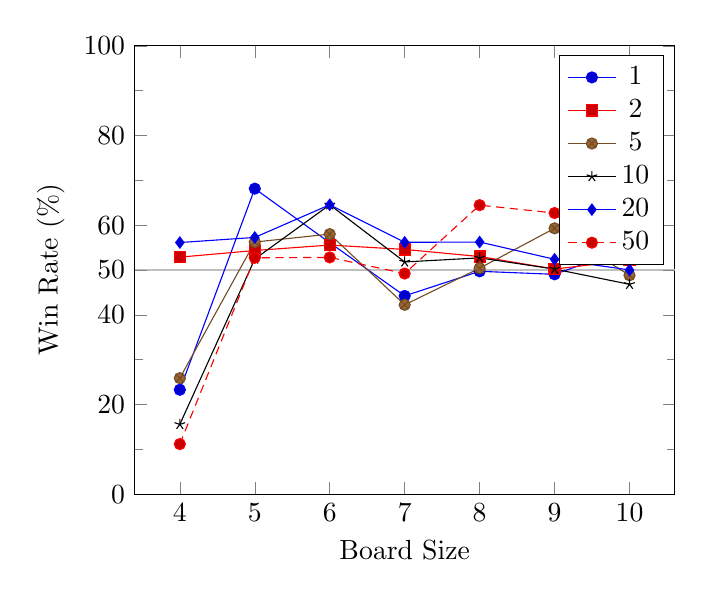
\begin{tikzpicture}
\begin{axis}[
	xlabel=Board Size,
	ylabel=Win Rate (\%),
	xtick={4,5,6,7,8,9,10},
	ymin=0, ymax=100,
	minor y tick num=1,
	extra y ticks={50},
	extra y tick style={grid=major},
]
%\addplot coordinates { (4,28.99) (5,54.56) (6,50.20) (7,48.39) (8,58.59) (9,56.05) (10,51.42) }; \addlegendentry{ 0.2}
%\addplot coordinates { (4,31.82) (5,58.78) (6,62.10) (7,56.27) (8,55.56) (9,56.05) (10,47.98) }; \addlegendentry{ 0.5}
\addplot coordinates { (4,23.28) (5,68.14) (6,56.08) (7,44.22) (8,49.70) (9,49.03) (10,54.98) }; \addlegendentry{ 1}
\addplot coordinates { (4,52.86) (5,54.34) (6,55.56) (7,54.58) (8,53.00) (9,50.20) (10,52.19) }; \addlegendentry{ 2}
\addplot coordinates { (4,25.87) (5,56.23) (6,58.00) (7,42.23) (8,50.40) (9,59.29) (10,48.81) }; \addlegendentry{ 5}
\addplot coordinates { (4,15.56) (5,52.44) (6,64.54) (7,51.79) (8,52.70) (9,50.20) (10,46.80) }; \addlegendentry{10}
\addplot coordinates { (4,56.12) (5,57.26) (6,64.54) (7,56.17) (8,56.23) (9,52.38) (10,50.00) }; \addlegendentry{20}
\addplot coordinates { (4,11.16) (5,52.72) (6,52.80) (7,49.20) (8,64.46) (9,62.70) (10,55.78) }; \addlegendentry{50}
\end{axis}
\end{tikzpicture}
	\caption[Edge Connectivity Bonus]{Edge Connectivity Bonus for Playing Near Groups that are Connected to an Edge or Corner Against Baseline RAVE Player}
	\label{fig:connectivity}
\end{figure}

Connecting to edges and corners is important for eventually winning the game, as most games end in a bridge or fork victory. Connecting to an edge is important, and extending groups that are already connected to an edge or corner is a good strategy for winning. The edges and corners that each group is connected to is already stored and updated for easy win detection. A bonus is given based on the number of edges or corners it is connected to. The maximum number of edges or corners a group could be connected to is 3, being 2 edges and 1 corner, so this gives a bonus between 0 and 3.

Figure \ref{fig:connectivity} shows the results. While no single value is strong on all board sizes, some value is strong on each board size, giving a winning rate between 55\% and 65\%, or 50 to 100 elo.



\subsection{Group Size}

\begin{figure}
	\centering
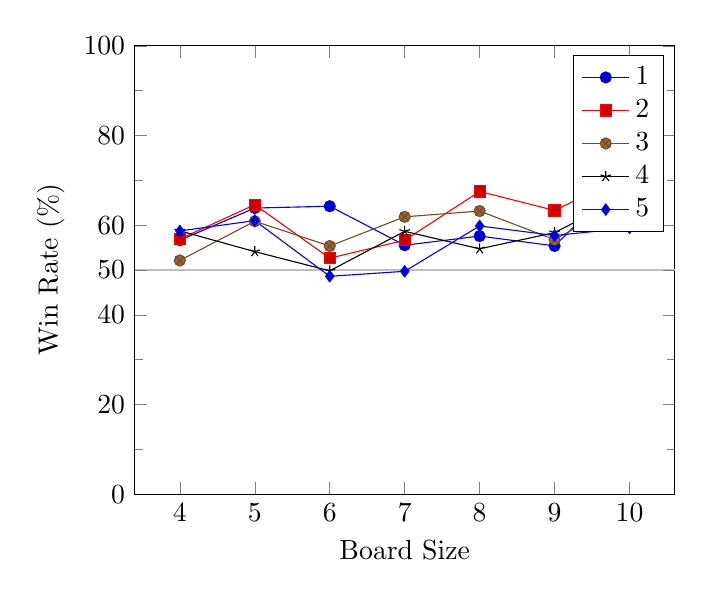
\begin{tikzpicture}
\begin{axis}[
	xlabel=Board Size,
	ylabel=Win Rate (\%),
	xtick={4,5,6,7,8,9,10},
	ymin=0, ymax=100,
	minor y tick num=1,
	extra y ticks={50},
	extra y tick style={grid=major},
]
\addplot coordinates { (4,56.63) (5,63.81) (6,64.22) (7,55.52) (8,57.56) (9,55.37) (10,71.92) }; \addlegendentry{  1}
\addplot coordinates { (4,56.92) (5,64.56) (6,52.63) (7,56.63) (8,67.51) (9,63.28) (10,71.43) }; \addlegendentry{  2}
\addplot coordinates { (4,52.12) (5,60.87) (6,55.34) (7,61.86) (8,63.14) (9,56.76) (10,66.04) }; \addlegendentry{  3}
\addplot coordinates { (4,58.73) (5,54.09) (6,49.81) (7,58.62) (8,54.72) (9,58.33) (10,66.87) }; \addlegendentry{  4}
\addplot coordinates { (4,58.70) (5,61.01) (6,48.59) (7,49.70) (8,59.82) (9,57.69) (10,59.39) }; \addlegendentry{  5}
%\addplot coordinates { (4,59.68) (5,61.13) (6,47.77) (7,55.72) (8,47.51) (9,45.58) (10,49.11) }; \addlegendentry{ 10}
%\addplot coordinates { (4,50.47) (5,42.84) (6,44.48) (7,50.43) (8,42.64) (9,44.92) (10,39.32) }; \addlegendentry{ 20}
%\addplot coordinates { (4,33.44) (5,42.65) (6,33.13) (7,40.36) (8,34.10) (9,28.88) (10,31.33) }; \addlegendentry{ 50}
%\addplot coordinates { (4,21.80) (5,30.79) (6,37.54) (7,30.45) (8,29.04) (9,19.21) (10,14.63) }; \addlegendentry{100}
%\addplot coordinates { (4,13.02) (5,20.64) (6,21.43) (7,14.37) (8,18.54) (9,9.71) (10,10.61) }; \addlegendentry{200}
\end{axis}
\end{tikzpicture}
	\caption[Group Size Bonus]{Group Size Bonus for Playing Near or Forming Big Groups Against Baseline RAVE Player}
	\label{fig:groupsize}
\end{figure}

Winning formations must span large sections of the board, and tend to be big. Letting a large group get cut off and made useless is rarely a winning strategy. Connecting smaller groups into larger groups is often a good idea. All of these suggest playing near and forming big groups, so here a bonus is given based on the size of the group. Placing a lone stone has no bonus. Joining two groups has a bonus equal to the sum of the sizes of the two groups. Joining a group has a bonus equal to the existing size of the group.

The results are shown in Figure \ref{fig:groupsize}. A winning rate over 60\% can be achieved on all board sizes.




\subsection{Distance to Win}\label{sec:distwin}

Most Havannah games end in either a bridge or a fork victory. It is possible to approximate the minimum number of moves needed to achieve these win conditions by doing a flood fill from each corner and edge, and counting the distance to each cell from the starting point. The distance between two cells that are part of the same group is counted as zero, since no additional stones are needed to connect them. The distance between any other neighbouring cells is one. Once the distances to each corner and edge are computed, the number of moves needed to achieve a victory from that cell is the sum of the shortest two distances to corners or the sum of the shortest three distances to edges. This method does not consider ring victories at all. It can over-estimate the number of moves since it doesn't consider that the paths to the corners or edges may share part of the path. It does not consider any moves by the opponent, which could easily increase the distance by blocking an essential move, or even make the connection impossible. It does not take virtual connections into account. All that said, it is a reasonable estimate in many cases. It is slow to compute, as it requires 12 flood fills for each player, but in doing so computes the minimum distance for every cell on the board. An example is shown in Figure \ref{fig:distances}, showing the minimum distances for white, black, and the minimum of the two. Note how the immediate threat has a distance of 1. White has low distances on the right where it dominates, while black has low distances on the left where it dominates.

\begin{figure}
	\centering
	\subfloat[]{\label{fig:distwhite}
		\begin{HavannahBoard}[board size=4,coordinate style=classical,show coordinates=false]
		\HGame[numbered moves=false]{a4,g4,a1,b3,g7,d1,d7,f3,e2,d2}
		\HStoneGroup[color=light gray,label=1]{}
		\HStoneGroup[color=light gray,label=2]{a2,a3,b5,c6,e7,f7}
		\HStoneGroup[color=light gray,label=3]{b1,b2,b4,c5,d6,e6,f6,g6}
		\HStoneGroup[color=light gray,label=4]{c3,c4,d5,e5}
		\HStoneGroup[color=light gray,label=5]{c1,c2,d4,f5,g5}
		\HStoneGroup[color=light gray,label=6]{d3,e3,e4,f4}
		\end{HavannahBoard}
	}
	\subfloat[]{\label{fig:distblack}
		\begin{HavannahBoard}[board size=4,coordinate style=classical,show coordinates=false]
		\HGame[numbered moves=false]{a4,g4,a1,b3,g7,d1,d7,f3,e2,d2}
		\HStoneGroup[color=light gray,label=1]{e3}
		\HStoneGroup[color=light gray,label=2]{c1,c2,d3,f4,g5}
		\HStoneGroup[color=light gray,label=3]{e4}
		\HStoneGroup[color=light gray,label=4]{b1,b2,c3,d4,f5,g6}
		\HStoneGroup[color=light gray,label=5]{a2,a3,b4,e5,f6}
		\HStoneGroup[color=light gray,label=6]{b5,c4,c5,c6,d5,d6,e6,e7,f7}
		\end{HavannahBoard}
	}
	\subfloat[]{\label{fig:distmin}
		\begin{HavannahBoard}[board size=4,coordinate style=classical,show coordinates=false]
		\HGame[numbered moves=false]{a4,g4,a1,b3,g7,d1,d7,f3,e2,d2}
		\HStoneGroup[color=light gray,label=1]{e3}
		\HStoneGroup[color=light gray,label=2]{a2,a3,b5,c1,c2,c6,d3,e7,f4,f7,g5}
		\HStoneGroup[color=light gray,label=3]{b1,b2,b4,c5,d6,e4,e6,f6,g6}
		\HStoneGroup[color=light gray,label=4]{c3,c4,d4,d5,e5,f5}
		\end{HavannahBoard}
	}
	\caption{Distance to a Win for (a) White (b) Black (c) Minimum of White and Black}
	\label{fig:distances}
\end{figure}


To turn this heuristic into usable knowledge, a small distance must give a larger bonus, while a large distance must give a small bonus. To accomplish this, the distance is subtracted from double of the board size, with a minimum value of zero.

First, using the minimum of the distances for the two players was tested, as in Figure \ref{fig:distmin}. This takes both offensive and defensive positions into account. The results are shown in Figure \ref{fig:distancetogether}. On smaller boards this method achieved a winning rate as high as 60\%, though failed to achieve any success on the bigger boards.

\begin{figure}
	\centering
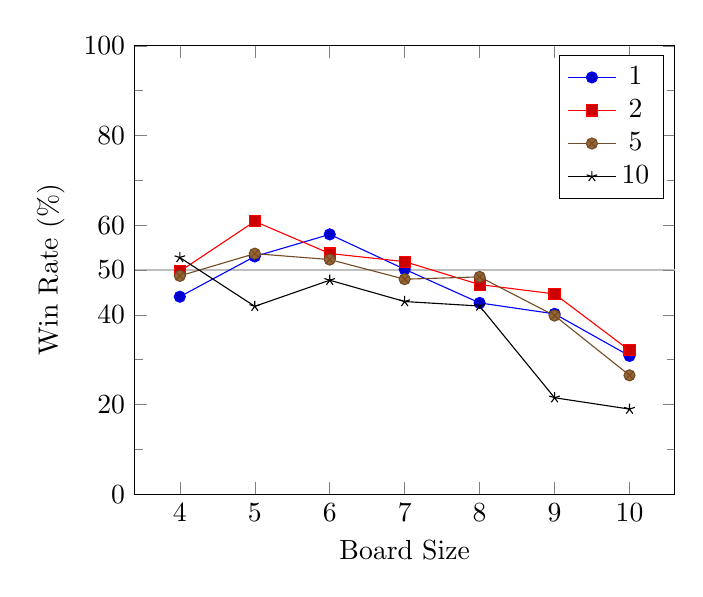
\begin{tikzpicture}
\begin{axis}[
	xlabel=Board Size,
	ylabel=Win Rate (\%),
	xtick={4,5,6,7,8,9,10},
	ymin=0, ymax=100,
	minor y tick num=1,
	extra y ticks={50},
	extra y tick style={grid=major},
]
\addplot coordinates { (4,44.04) (5,53.01) (6,57.94) (7,50.16) (8,42.65) (9,40.21) (10,30.83) }; \addlegendentry{  1}
\addplot coordinates { (4,49.69) (5,60.84) (6,53.67) (7,51.86) (8,46.74) (9,44.66) (10,32.06) }; \addlegendentry{  2}
%\addplot coordinates { (4,50.54) (5,59.89) (6,54.69) (7,52.77) (8,49.39) (9,39.27) (10,30.13) }; \addlegendentry{  3}
%\addplot coordinates { (4,50.31) (5,57.19) (6,58.67) (7,51.14) (8,48.53) (9,38.66) (10,29.20) }; \addlegendentry{  4}
\addplot coordinates { (4,48.68) (5,53.64) (6,52.32) (7,47.94) (8,48.46) (9,39.82) (10,26.50) }; \addlegendentry{  5}
\addplot coordinates { (4,52.78) (5,41.89) (6,47.71) (7,42.96) (8,41.96) (9,21.50) (10,18.97) }; \addlegendentry{ 10}
%\addplot coordinates { (4,32.22) (5,32.35) (6,37.18) (7,35.24) (8,30.69) (9,18.75) (10,17.44) }; \addlegendentry{ 20}
%\addplot coordinates { (4,10.00) (5,23.33) (6,19.67) (7,25.26) (8,16.30) (9,8.70) (10,6.14) }; \addlegendentry{ 50}
%\addplot coordinates { (4,6.56) (5,13.64) (6,15.19) (7,11.32) (8,12.93) (9,15.79) (10,12.50) }; \addlegendentry{100}
%\addplot coordinates { (4,2.27) (5,10.77) (6,12.68) (7,5.75) (8,16.87) (9,23.29) (10,10.71) }; \addlegendentry{200}
\end{axis}
\end{tikzpicture}
	\caption[Minimum Distance to Win Bonus]{Minimum Distance to Win Bonus Against Baseline RAVE Player}
	\label{fig:distancetogether}
\end{figure}


Next, using only the distance for the current player was tested, as in Figures \ref{fig:distwhite} and \ref{fig:distblack}. This is a much more offensive metric, ignoring the opponent's distance to win. The results are shown in Figure \ref{fig:distancesides}. This method achieves especially good results on small boards with a winning rate as high as 70\%, but achieved positive results up to size 9.

\begin{figure}
	\centering
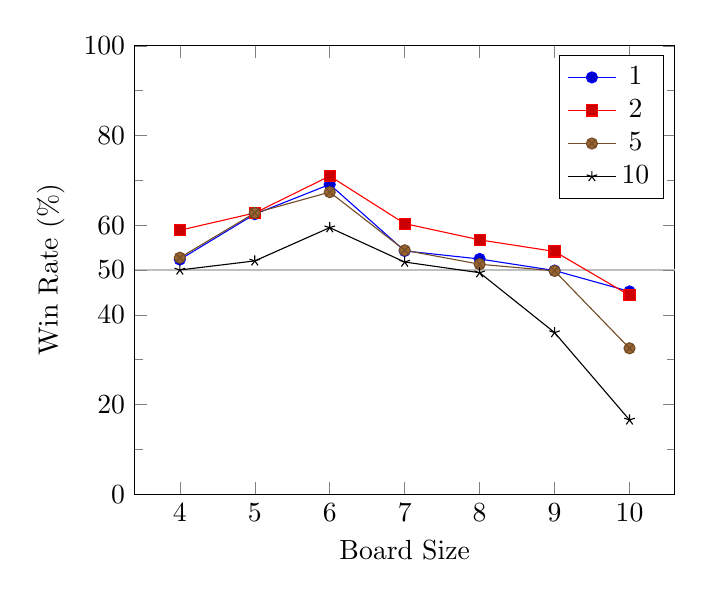
\begin{tikzpicture}
\begin{axis}[
	xlabel=Board Size,
	ylabel=Win Rate (\%),
	xtick={4,5,6,7,8,9,10},
	ymin=0, ymax=100,
	minor y tick num=1,
	extra y ticks={50},
	extra y tick style={grid=major},
]
\addplot coordinates { (4,52.33) (5,62.45) (6,69.08) (7,54.25) (8,52.45) (9,49.87) (10,45.21) }; \addlegendentry{ 1}
\addplot coordinates { (4,58.86) (5,62.72) (6,70.95) (7,60.34) (8,56.72) (9,54.13) (10,44.33) }; \addlegendentry{ 2}
%\addplot coordinates { (4,54.02) (5,62.36) (6,63.20) (7,58.46) (8,57.03) (9,53.03) (10,42.02) }; \addlegendentry{ 3}
%\addplot coordinates { (4,44.30) (5,57.25) (6,61.73) (7,59.86) (8,58.20) (9,53.98) (10,41.07) }; \addlegendentry{ 4}
\addplot coordinates { (4,52.74) (5,62.72) (6,67.36) (7,54.39) (8,51.28) (9,49.79) (10,32.53) }; \addlegendentry{ 5}
\addplot coordinates { (4,50.00) (5,52.02) (6,59.44) (7,51.77) (8,49.39) (9,36.04) (10,16.55) }; \addlegendentry{10}
\end{axis}
\end{tikzpicture}
	\caption[Own Minimum Distance to Win]{Own Minimum Distance to Win Bonus Against Baseline RAVE Player}
	\label{fig:distancesides}
\end{figure}


\section{Rollout Policy}

The other main way to improve MCTS is by changing the move choice in rollouts so that the outcome of the rollouts is more representative of the real strength of the position. Usually this means using simple patterns or heuristics to make moves that are more sensible than choosing moves randomly.

\subsection{Mate-in-one}

If the opportunity to win with a single move (mate-in-one) exists, a smart player would make that move. Similarly, if the opponent has a threat to win in a single move, a smart player would block that move. Lorentz tested mate-in-one checks, and the defensive variant, to great success. Fossel also tested mate-in-one checks achieving a 59\% win rate on size 5 with equal time\cite{fossel2010monte}. Because checking for win conditions is a slow operation, both Lorentz and Fossel achieved the greatest success when limiting the checks to only the first few moves of the rollout, where they are most representative of the true board state.

Mate-in-one checks are very slow. The obvious way of implementing it is to check every empty cell for each player for whether a move there would complete a win condition. This is $O(n)$ of the number of cells, which makes rollouts $O(n^2)$. A simple optimization is to only do the win check if that cell is next to an existing stone, but this is still $O(n)$. A much better algorithm is to only do win checks on the empty cells next to the group that was last played, which is roughly $O(g)$ where $g$ is the group size and $g \ll n$. This works because we are making the assertion that no mate-in-one moves exists before the last move, and so a new mate-in-one must be related to the last played stone. If the last played stone creates one new winning cell, we must block it. If it creates two new winning cells, it has a guaranteed win, and so we just end the rollout early. Castro does not have a facility to enumerate the empty cells surrounding a group, so instead it does a walk around the group. There must be a position around the cell that is not part of the same group, even if it is off the board. If this was not true, then it would be in the center of a ring, and the game would already be finished. It then follows the edge of the group, checking only whether placing an additional stone in the neighbouring empty cells would turn that group into a winning structure. The walk ends when it gets back to the first position searched. An additional untested optimization would be to only do this check if the last placed stone has a connection to an edge or corner, though this ignores ring threats.

We tested checking for mate-in-one moves after every move, and limiting the checks to only to the first N moves with N equal to the board size and double the board size. The results are shown in Figure \ref{fig:mateinone}. The best result is achieved exactly where Lorentz and Fossel reported their success, on size 5, but all other cases were inconclusive or quite negative. Discussions with other Havannah programmers suggested mate-in-one checks become more important as the time per move is increased, so size and size*2 were tested with 30 seconds per move, with the results shown in Figure \ref{fig:mateinone30}. The results are more promising, but do have bigger confidence intervals due to the time consuming process of testing such long games.

\begin{figure}
	\centering
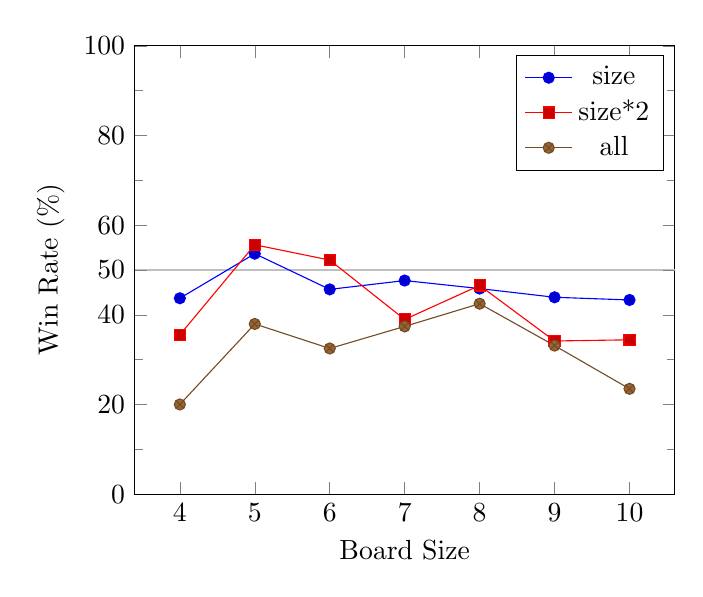
\begin{tikzpicture}
\begin{axis}[
	xlabel=Board Size,
	ylabel=Win Rate (\%),
	xtick={4,5,6,7,8,9,10},
	ymin=0, ymax=100,
	minor y tick num=1,
	extra y ticks={50},
	extra y tick style={grid=major},
]
%\addplot coordinates { (4,54.26) (5,47.92) (6,43.78) (7,49.27) (8,51.75) (9,46.91) (10,50.58) }; \addlegendentry{2}
%\addplot coordinates { (4,48.75) (5,57.66) (6,53.06) (7,49.32) (8,44.49) (9,44.85) (10,48.77) }; \addlegendentry{5}
%\addplot coordinates { (4,27.78) (5,54.42) (6,48.87) (7,44.27) (8,40.97) (9,45.27) (10,46.71) }; \addlegendentry{10}
\addplot coordinates { (4,43.69) (5,53.63) (6,45.67) (7,47.64) (8,45.85) (9,43.91) (10,43.31) }; \addlegendentry{size}
\addplot coordinates { (4,35.53) (5,55.62) (6,52.21) (7,38.96) (8,46.55) (9,34.16) (10,34.42) }; \addlegendentry{size*2}
\addplot coordinates { (4,20.00) (5,37.96) (6,32.49) (7,37.41) (8,42.48) (9,33.13) (10,23.49) }; \addlegendentry{all}
\end{axis}
\end{tikzpicture}
	\caption{Mate-in-one Checking Against Baseline RAVE Player With 5 Seconds per Move}
	\label{fig:mateinone}
\end{figure}

\begin{figure}
	\centering
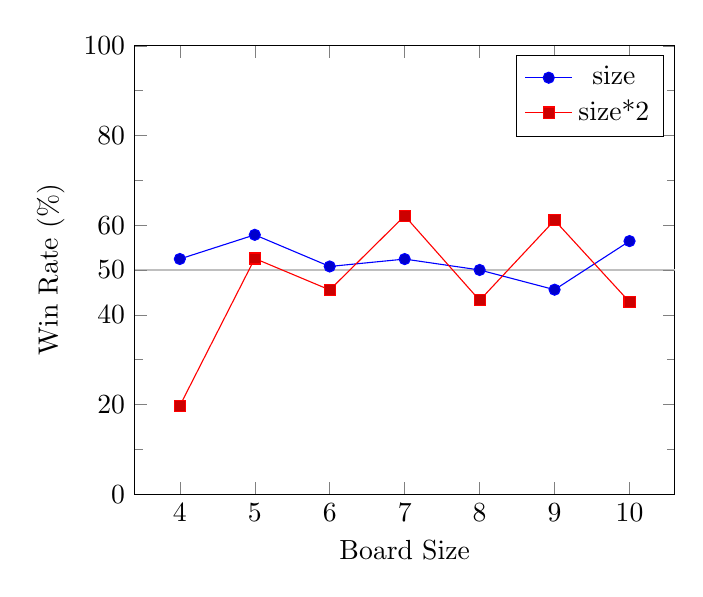
\begin{tikzpicture}
\begin{axis}[
	xlabel=Board Size,
	ylabel=Win Rate (\%),
	xtick={4,5,6,7,8,9,10},
	ymin=0, ymax=100,
	minor y tick num=1,
	extra y ticks={50},
	extra y tick style={grid=major},
]
%\addplot coordinates { (4,63.33) (5,52.10) (6,52.51) (7,56.13) (8,50.23) (9,41.24) (10,46.98) }; \addlegendentry{2}
%\addplot coordinates { (4,54.50) (5,51.43) (6,54.09) (7,56.87) (8,41.92) (9,51.84) (10,44.55) }; \addlegendentry{5}
%\addplot coordinates { (4,1.47) (5,52.05) (6,60.47) (7,50.73) (8,46.93) (9,52.16) (10,53.92) }; \addlegendentry{10}
\addplot coordinates { (4,52.45) (5,57.84) (6,50.78) (7,52.43) (8,50.00) (9,45.60) (10,56.44) }; \addlegendentry{size}
\addplot coordinates { (4,19.72) (5,52.56) (6,45.55) (7,62.08) (8,43.22) (9,61.09) (10,42.86) }; \addlegendentry{size*2}
\end{axis}
\end{tikzpicture}
	\caption{Mate-in-one Checking Against Baseline RAVE Player With 30 Seconds per Move}
	\label{fig:mateinone30}
\end{figure}

\subsection{Maintain Virtual Connection}

Maintaining virtual connections is important, as chains of virtual connections can form frames that, when completed, form a winning condition. If an opponent places a stone in one of the two parts of a VC, the response should be to reply in the remaining empty position that used to form the VC. This can be implemented with a small state machine looking at the neighbours to the last placed stone, looking for the pattern of your stone, empty, your stone. If this pattern is found, the empty cell between your two stones is the correct response to maintain the virtual connection. Maintaining a connection to an edge is also important, so the pattern still works if either of your stones is off the edge of the board, as in your stone, empty, off the board. This pattern is checked after every move. If no pattern is found, then the default policy is used, resulting in a random move being chosen.

Looking for this pattern is extremely fast, causing no slowdown in terms of simulations per second. The time taken for the pattern lookup is offset by the approximately 10\% shorter rollouts. The results are shown in Figure \ref{fig:maintainvcrollout}, showing a negligible or even negative result.

\begin{figure}
	\centering
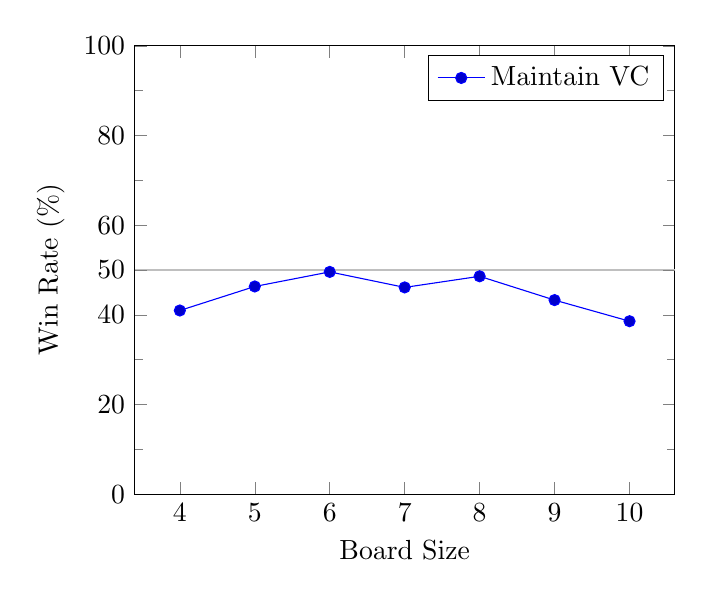
\begin{tikzpicture}
\begin{axis}[
	xlabel=Board Size,
	ylabel=Win Rate (\%),
	xtick={4,5,6,7,8,9,10},
	ymin=0, ymax=100,
	minor y tick num=1,
	extra y ticks={50},
	extra y tick style={grid=major},
]
\addplot coordinates { (4,40.96) (5,46.32) (6,49.57) (7,46.11) (8,48.59) (9,43.28) (10,38.57) }; \addlegendentry{Maintain VC}
\end{axis}
\end{tikzpicture}
	\caption{Maintain Virtual Connections in the Rollout Against Baseline RAVE Player}
	\label{fig:maintainvcrollout}
\end{figure}

\subsection{Last Good Reply}

Last Good Reply (LGR) is a game-independent method of improving the moves in a rollout by taking advantage of local situations. It attempts to reuse good moves in later rollouts by saving all the replies by the winning player and forcing the reply in later simulations if the reply is valid.

LGR only saves the replies to individual moves. If a good reply is known to the opponent's last move, it is made instead of a random move. If that move is invalid, a random move is made instead.

If a reply was played, but the outcome of the rollout is a loss, that may not be such a good move, and so it should be forgotten. This variant, called Last Good Reply with Forgetting (LGRF) removes the replies for all the moves made by the losing player. This increases the amount of randomness in the rollouts as compared to LGR.

Figure \ref{fig:lgr} shows the results. LGR only works on size 4, while LGRF is helpful on sizes 6 and up, leading to a 50-100 elo performance gain.

\begin{figure}
	\centering
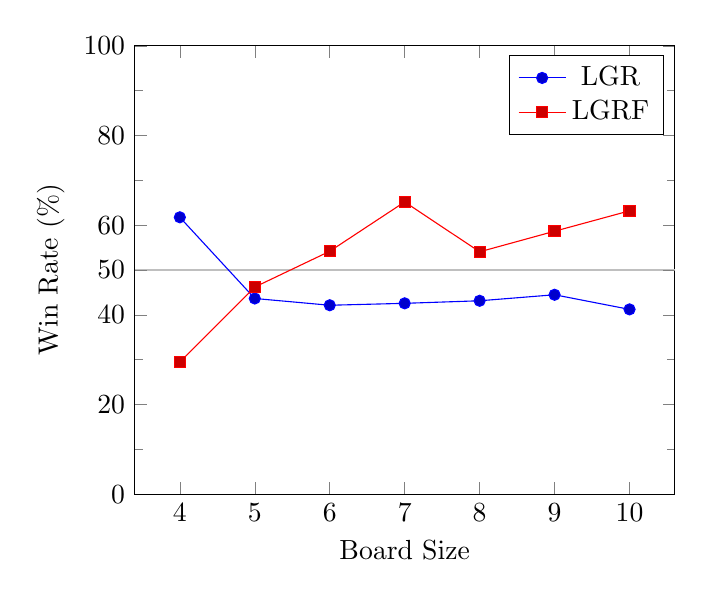
\begin{tikzpicture}
\begin{axis}[
	xlabel=Board Size,
	ylabel=Win Rate (\%),
	xtick={4,5,6,7,8,9,10},
	ymin=0, ymax=100,
	minor y tick num=1,
	extra y ticks={50},
	extra y tick style={grid=major},
]
\addplot coordinates { (4,61.75) (5,43.64) (6,42.13) (7,42.56) (8,43.13) (9,44.47) (10,41.21) }; \addlegendentry{LGR}
\addplot coordinates { (4,29.45) (5,46.19) (6,54.17) (7,65.18) (8,54.05) (9,58.64) (10,63.19) }; \addlegendentry{LGRF}
\end{axis}
\end{tikzpicture}
	\caption{Last Good Reply Against Baseline RAVE Player}
	\label{fig:lgr}
\end{figure}


\subsection{Ring Rule Variations}\label{sec:ringrules}

The three win conditions happen at different frequencies on different board sizes, as shown in Table \ref{tab:wintypes}. On size 4, a bridge is the most frequent win type followed by fork and the relatively infrequent ring victory. As the board size increases, it becomes harder for bridges and forks to form as they scale with the size of the board, but rings become relatively easier, because their size is independent of the board size and they are local formations. Given empty space on the board, a ring is likely to occur purely by making random moves. Rings are quite easy to block however, so while they happen frequently in random games, they are rare in real games. MCTS is very sensitive to the outcome of rollouts not being representative of the strength of the starting position, so this mismatch is a problem.

\begin{table}
	\centering
	\begin{tabular}{l|rrr}
		Size & Fork & Bridge & Ring \\ \hline
		   4 & 4267 &   5177 &  543 \\
		   5 & 5111 &   2962 & 1926 \\
		   6 & 4471 &   1691 & 3838 \\
		   7 & 3536 &   1007 & 5457 \\
		   8 & 2266 &    460 & 7274 \\
		   9 & 1365 &    229 & 8406 \\
		   10 & 796 &    126 & 9078 \\
	\end{tabular}
	\caption{Number of Wins of Each Type by Board Size Given 10000 Simulations}
	\label{tab:wintypes}
\end{table}

Four different solutions to this problem were explored. Instead of modifying where stones are placed, the rules of the game are modified. If a ring is formed, but the modified rules deem it to be a product of randomness instead of the product of good strategy, it is simply ignored and the rollout continues until a different winning condition occurs. Note that this only affects rings formed during rollouts. If the tree reaches a position with a ring, it is still considered a win regardless of the rule modifications considered here.

\subsubsection{Ignore all rings}

\begin{figure}
	\centering
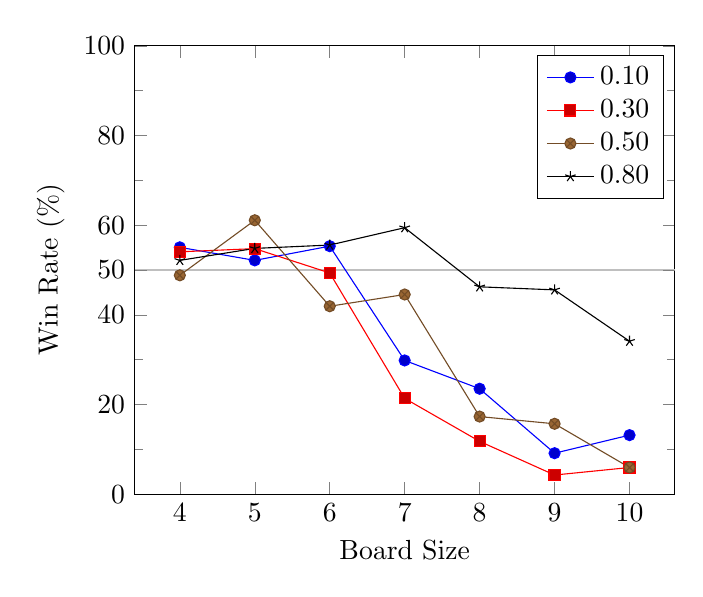
\begin{tikzpicture}
\begin{axis}[
	xlabel=Board Size,
	ylabel=Win Rate (\%),
	xtick={4,5,6,7,8,9,10},
	ymin=0, ymax=100,
	minor y tick num=1,
	extra y ticks={50},
	extra y tick style={grid=major},
]
%\addplot coordinates { (4,57.69) (5,53.65) (6,49.08) (7,29.83) (8,4.83) (9,5.26) (10,15.16) }; \addlegendentry{0.05}
\addplot coordinates { (4,55.05) (5,52.14) (6,55.31) (7,29.82) (8,23.51) (9,9.13) (10,13.16) }; \addlegendentry{0.10}
%\addplot coordinates { (4,55.47) (5,55.16) (6,56.65) (7,26.76) (8,8.33) (9,4.22) (10,12.45) }; \addlegendentry{0.20}
\addplot coordinates { (4,54.05) (5,54.76) (6,49.33) (7,21.36) (8,11.77) (9,4.26) (10,5.94) }; \addlegendentry{0.30}
\addplot coordinates { (4,48.81) (5,61.09) (6,41.91) (7,44.53) (8,17.30) (9,15.69) (10,5.94) }; \addlegendentry{0.50}
\addplot coordinates { (4,52.14) (5,54.81) (6,55.56) (7,59.43) (8,46.24) (9,45.56) (10,34.11) }; \addlegendentry{0.80}
\end{axis}
\end{tikzpicture}
	\caption{Ring Rule Ignore Rings Against Baseline RAVE Player}
	\label{fig:ringignore}
\end{figure}

The simplest rule modification is to simply ignore all occurrences of rings during some fraction of the rollouts. At the beginning of the rollout a random number is generated and if it is below the configurable fraction, rings are checked, otherwise all rings are ignored.

The results are shown in Figure \ref{fig:ringignore}. There are minor successes on smaller boards, but bad results on bigger boards where rings are a problem. The bad results happen because it completely misses the opponent's real and faster ring threats, instead focusing on its own slower bridge and fork victories. By the time it notices the opponent's rings, it is too late to block them. This effect may be less pronounced against human opponents that are less likely to make ring threats, but it would introduce a new weakness that could be exploited.



\subsubsection{Fixed depth}

\begin{table}
	\centering
	\begin{tabular}{l|rrr}
		Size & Fork   & Bridge &   Ring \\ \hline
		   4 &  29.56 &  26.34 &  28.00 \\
		   5 &  48.13 &  44.77 &  44.36 \\
		   6 &  71.66 &  68.01 &  65.07 \\
		   7 &  98.91 &  93.74 &  89.14 \\
		   8 & 131.29 & 126.29 & 116.38 \\
		   9 & 167.01 & 160.12 & 146.13 \\
		  10 & 206.35 & 196.88 & 177.64 \\
	\end{tabular}
	\caption{Average Number of Moves in a Rollout Before Each Victory Type}
	\label{tab:wintypedepth}
\end{table}

\begin{figure}
	\centering
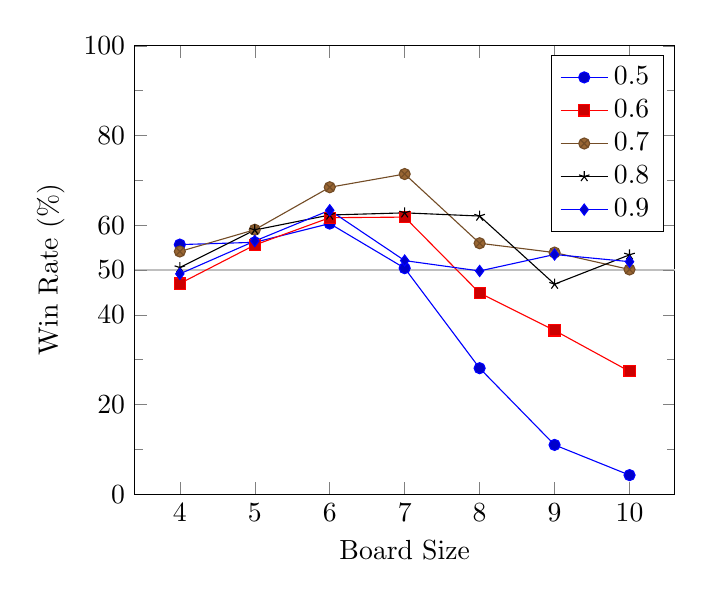
\begin{tikzpicture}
\begin{axis}[
	xlabel=Board Size,
	ylabel=Win Rate (\%),
	xtick={4,5,6,7,8,9,10},
	ymin=0, ymax=100,
	minor y tick num=1,
	extra y ticks={50},
	extra y tick style={grid=major},
]
%\addplot coordinates { (4,51.37) (5,51.77) (6,48.62) (7,30.49) (8,8.21) (9,2.99) (10,5.46) }; \addlegendentry{0.2}
%\addplot coordinates { (4,45.51) (5,55.66) (6,49.71) (7,32.30) (8,10.31) (9,4.23) (10,5.72) }; \addlegendentry{0.3}
%\addplot coordinates { (4,53.69) (5,50.77) (6,53.67) (7,37.78) (8,15.31) (9,3.96) (10,10.99) }; \addlegendentry{0.4}
\addplot coordinates { (4,55.66) (5,56.17) (6,60.35) (7,50.40) (8,28.09) (9,10.98) (10,4.24) }; \addlegendentry{0.5}
\addplot coordinates { (4,46.97) (5,55.57) (6,61.66) (7,61.79) (8,44.86) (9,36.51) (10,27.38) }; \addlegendentry{0.6}
\addplot coordinates { (4,54.12) (5,58.98) (6,68.45) (7,71.40) (8,55.96) (9,53.88) (10,50.11) }; \addlegendentry{0.7}
\addplot coordinates { (4,50.54) (5,58.92) (6,62.26) (7,62.74) (8,62.03) (9,46.84) (10,53.37) }; \addlegendentry{0.8}
\addplot coordinates { (4,49.13) (5,56.45) (6,63.32) (7,52.09) (8,49.78) (9,53.45) (10,51.85) }; \addlegendentry{0.9}

\end{axis}
\end{tikzpicture}
	\caption{Ring Rule Fixed Depth Against Baseline RAVE Player}
	\label{fig:ringdepth}
\end{figure}

Table \ref{tab:wintypedepth} shows the number of moves before each win condition is achieved, showing that rings occur the earliest, especially on big boards. This is expected due to their smaller size and being local properites. If instead of ignoring all rings, we allow rings for the first part of the rollout and ignore all rings after that cutoff, we may allow legitimate ring threats while ignoring rings that occur purely due to randomness. As the board size increases, this depth should also be increased, so instead of an absolute value, we use a fraction of the number of empty cells on the board at the beginning of the rollout.

The results are shown in Figure \ref{fig:ringdepth}, showing results as high as a 71\% winning rate for only considering rings until 70\% of the empty cells are played. The benefits on board sizes 8, 9 and 10 are still quite small though, where the problem is the worst.


\subsubsection{Ring size}

\begin{figure}
	\centering
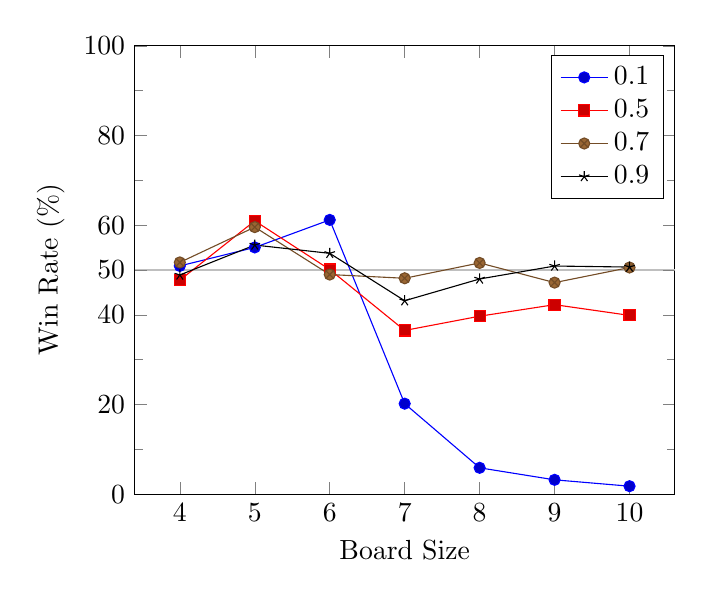
\begin{tikzpicture}
\begin{axis}[
	xlabel=Board Size,
	ylabel=Win Rate (\%),
	xtick={4,5,6,7,8,9,10},
	ymin=0, ymax=100,
	minor y tick num=1,
	extra y ticks={50},
	extra y tick style={grid=major},
]
\addplot coordinates { (4,50.90) (5,55.03) (6,61.17) (7,20.18) (8,5.87) (9,3.19) (10,1.77) }; \addlegendentry{0.1}
%\addplot coordinates { (4,50.00) (5,61.72) (6,51.25) (7,32.39) (8,19.07) (9,14.60) (10,10.09) }; \addlegendentry{0.2}
%\addplot coordinates { (4,49.77) (5,61.53) (6,48.34) (7,40.72) (8,30.29) (9,29.09) (10,23.42) }; \addlegendentry{0.3}
%\addplot coordinates { (4,48.70) (5,59.83) (6,48.68) (7,34.78) (8,34.75) (9,34.83) (10,34.55) }; \addlegendentry{0.4}
\addplot coordinates { (4,47.72) (5,60.96) (6,50.10) (7,36.51) (8,39.69) (9,42.26) (10,39.87) }; \addlegendentry{0.5}
%\addplot coordinates { (4,53.77) (5,59.07) (6,51.52) (7,39.36) (8,47.18) (9,43.13) (10,48.96) }; \addlegendentry{0.6}
\addplot coordinates { (4,51.69) (5,59.56) (6,48.98) (7,48.15) (8,51.57) (9,47.18) (10,50.55) }; \addlegendentry{0.7}
%\addplot coordinates { (4,52.63) (5,59.08) (6,55.43) (7,45.91) (8,48.09) (9,53.45) (10,54.55) }; \addlegendentry{0.8}
\addplot coordinates { (4,48.88) (5,55.56) (6,53.71) (7,43.14) (8,47.99) (9,50.88) (10,50.65) }; \addlegendentry{0.9}
\end{axis}
\end{tikzpicture}
	\caption{Ring Rule Ring Size Against Baseline RAVE Player}
	\label{fig:ringsize}
\end{figure}

The most commonly occuring ring  is the simple size 6 ring, which is easy to block. We may want to allow larger rings while still ignoring the easy to block 6 ring. Using the search-based ring check described in Section \ref{sec:ringimpl}, we can ignore rings smaller than a minimum value. In this test we start by allowing all rings, and after every N moves, we increase the minimum size by 1 for variable N. After the first N this would imply only rings of size 7 or bigger, then 8 or bigger, etc. Here we set N as a fraction of the remaining empty cells.

The results are shown in Figure \ref{fig:ringsize}, again showing reasonable results on board sizes 5 and 6 with a winning rate of 60\%, but failing to show any improvement on larger board sizes. A fraction of 0.7 or 0.9 is so high that it never reaches a minimum size bigger than 7, though this is enough to ignore size 6 rings.



\subsubsection{Permanent stones}

\begin{figure}
	\centering
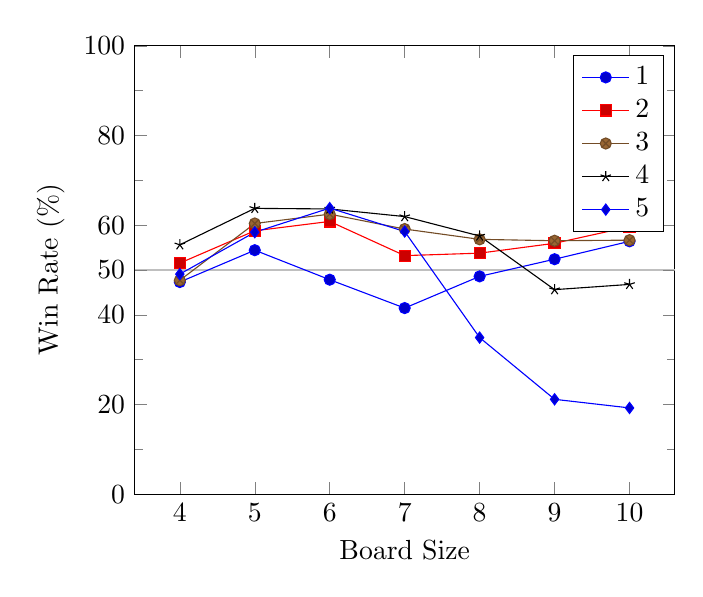
\begin{tikzpicture}
\begin{axis}[
	xlabel=Board Size,
	ylabel=Win Rate (\%),
	xtick={4,5,6,7,8,9,10},
	ymin=0, ymax=100,
	minor y tick num=1,
	extra y ticks={50},
	extra y tick style={grid=major},
]
\addplot coordinates { (4,47.31) (5,54.41) (6,47.83) (7,41.50) (8,48.57) (9,52.40) (10,56.39) }; \addlegendentry{1}
\addplot coordinates { (4,51.53) (5,58.74) (6,60.83) (7,53.20) (8,53.75) (9,55.95) (10,59.65) }; \addlegendentry{2}
\addplot coordinates { (4,47.70) (5,60.37) (6,62.45) (7,59.13) (8,56.83) (9,56.52) (10,56.65) }; \addlegendentry{3}
\addplot coordinates { (4,55.62) (5,63.74) (6,63.61) (7,61.91) (8,57.58) (9,45.61) (10,46.78) }; \addlegendentry{4}
\addplot coordinates { (4,49.08) (5,58.42) (6,63.80) (7,58.58) (8,34.92) (9,21.15) (10,19.23) }; \addlegendentry{5}
\end{axis}
\end{tikzpicture}
	\caption{Ring Rule Permanent Stones Against Baseline RAVE Player}
	\label{fig:ringperm}
\end{figure}

If the problem is that random moves form rings in empty parts of the board, a solution may be to only consider rings that include stones that exist on the board before the rollout begins. Thus ring threats may be formed from existing stones, but not purely out of randomness with little relation to the stones already existing on the board. In this test, stones that exist before the rollout begins are marked as permanent stones, and any ring found during the rollout must have a minimum number of permanent stones to be considered a winning formation. Requiring between 1 and 5 permanent stones was tested, with the results shown in Figure \ref{fig:ringperm}. This shows a 50-100 elo gain on all board sizes. In human play it makes reasonable ring threats, but is no longer fixated on rings.


\begin{table}
	\centering
	\begin{tabular}{l|rrr}
		Size & Fork & Bridge & Ring \\ \hline
		   4 & 4212 &   5644 & 136 \\
		   5 & 5986 &   3773 & 236 \\
		   6 & 7051 &   2321 & 626 \\
		   7 & 7444 &   2132 & 422 \\
		   8 & 8283 &   1397 & 319 \\
		   9 & 8635 &    929 & 436 \\
		  10 & 8768 &    971 & 261 \\
	\end{tabular}
	\caption{Number of Wins of Each Type by Board Size Given 10000 Simulations When Only Counting Rings With Three or More Permanent Stones}
	\label{tab:wintypesperm}
\end{table}

The results of using this feature when requiring a minimum of 3 permanent stones are shown in Table \ref{tab:wintypesperm}, and show a stark contrast to Table \ref{tab:wintypes} when not using this feature. The number of forks increases quite dramatically as the board size increases, especially relative to without this feature. This is expected due to the increasing amount of edges available, and the proportionately smaller increase in the number of stones needed to form a fork. The number of bridges decreases as the board size increases, as is expected since the number of corners is fixed but the distance between them is larger. Note how the decrease is not as dramatic as without this feature. The ring rate, however, drops dramatically compared to without this feature, and stays a fairly stable 2-6\% of all wins across board sizes. This is a much more reasonable number when starting from an empty board, given that rings have almost no strategic value.

\section{Combinations}

To show that these features combine, all of the features that showed positive results were combined into a single test case, and then single features were removed. All of these test cases were then tested against the same RAVE baseline as all the other tests were tested against. The heuristic knowledge features and rollout policy features are shown in separate graphs for clarity, but the test case marked `All' is identical on these two graphs.

The heuristic knowledge features that were included are:
\begin{itemize}
\item Maintain Virtual Connections (value 100)
\item Connectivity (value 20)
\item Locality (value 3)
\item Local Reply (value 5)
\item Distance (value 2)
\item Group Size (value 2)
\end{itemize}

The rollout policy features that were included are:
\begin{itemize}
\item Multiple rollouts (5 rollouts per simulation)
\item Mate-in-one (Only for the first N moves where N is the board size)
\item Ring Rule Depth (Only allow rings until 70\% of empty cells are filled)
\item Ring Rule Permanent Stones (Rings require 3 permanent stones)
\end{itemize}



\begin{figure}
	\centering
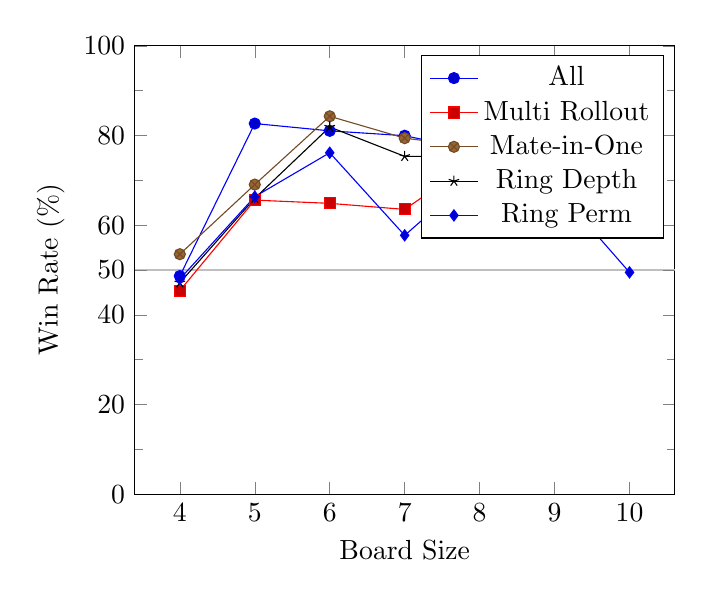
\begin{tikzpicture}
\begin{axis}[
	xlabel=Board Size,
	ylabel=Win Rate (\%),
	xtick={4,5,6,7,8,9,10},
	ymin=0, ymax=100,
	minor y tick num=1,
	extra y ticks={50},
	extra y tick style={grid=major},
]
\addplot coordinates { (4,48.65) (5,82.66) (6,81.03) (7,79.95) (8,76.49) (9,74.25) (10,64.88) }; \addlegendentry{All}
\addplot coordinates { (4,45.39) (5,65.58) (6,64.86) (7,63.51) (8,75.07) (9,69.38) (10,67.21) }; \addlegendentry{Multi Rollout}
\addplot coordinates { (4,53.52) (5,69.05) (6,84.28) (7,79.40) (8,77.30) (9,69.11) (10,67.38) }; \addlegendentry{Mate-in-One}
\addplot coordinates { (4,47.15) (5,65.99) (6,81.89) (7,75.34) (8,75.40) (9,70.16) (10,71.35) }; \addlegendentry{Ring Depth}
\addplot coordinates { (4,47.98) (5,66.35) (6,76.15) (7,57.72) (8,72.36) (9,68.56) (10,49.46) }; \addlegendentry{Ring Perm}
\end{axis}
\end{tikzpicture}
	\caption{Rollout Modifications}
	\label{fig:comborollout}
\end{figure}


The rollout policy related features are shown in Figure \ref{fig:comborollout}. Removing the multiple rollout feature causes a big drop in performance on board sizes 5-7, but little impact elsewhere. Removing mate-in-one checking or the ring depth causes a drop in performance on size 5, but no where else. The most dramatic difference is the removal of the permanent stones ring rule modification. Removing that feature causes a drop on board sizes 5-10, with particularly big drops on board sizes 5, 7 and 10. The permanent stone ring rule modification likely makes the heuristic knowledge features much more effective on the bigger board sizes. None of these features appear to have much affect on size 4.


\begin{figure}
	\centering
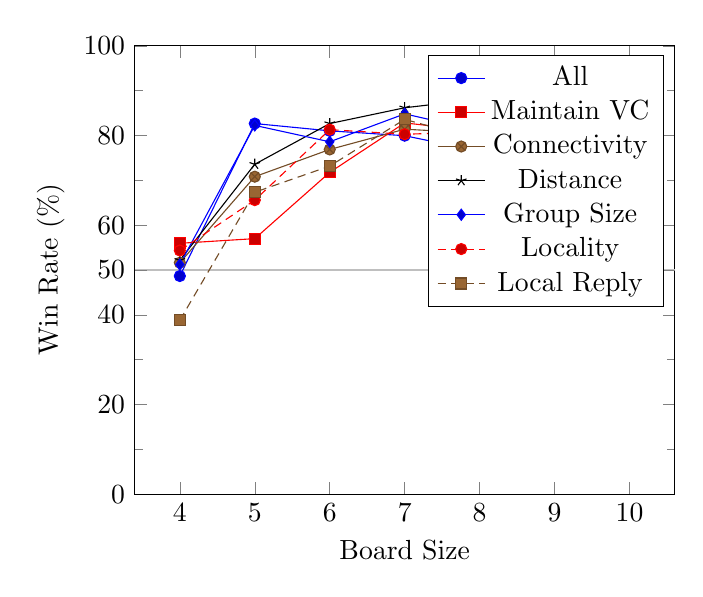
\begin{tikzpicture}
\begin{axis}[
	xlabel=Board Size,
	ylabel=Win Rate (\%),
	xtick={4,5,6,7,8,9,10},
	ymin=0, ymax=100,
	minor y tick num=1,
	extra y ticks={50},
	extra y tick style={grid=major},
]
\addplot coordinates { (4,48.65) (5,82.66) (6,81.03) (7,79.95) (8,76.49) (9,74.25) (10,64.88) }; \addlegendentry{All}
\addplot coordinates { (4,55.95) (5,56.99) (6,71.77) (7,82.80) (8,80.93) (9,72.39) (10,68.62) }; \addlegendentry{Maintain VC }
\addplot coordinates { (4,51.62) (5,70.81) (6,76.88) (7,81.40) (8,80.49) (9,73.98) (10,79.40) }; \addlegendentry{Connectivity}
\addplot coordinates { (4,52.17) (5,73.58) (6,82.66) (7,86.18) (8,88.14) (9,80.32) (10,83.07) }; \addlegendentry{Distance}
\addplot coordinates { (4,51.22) (5,82.25) (6,78.59) (7,84.82) (8,81.02) (9,75.93) (10,66.31) }; \addlegendentry{Group Size}
\addplot coordinates { (4,54.34) (5,65.58) (6,81.30) (7,80.27) (8,80.81) (9,78.92) (10,73.32) }; \addlegendentry{Locality}
\addplot coordinates { (4,38.78) (5,67.34) (6,73.17) (7,83.60) (8,78.98) (9,79.78) (10,69.54) }; \addlegendentry{Local Reply}
\end{axis}
\end{tikzpicture}
	\caption{Knowledge Modifications}
	\label{fig:comboknow}
\end{figure}

The knowledge heuristic features are shown in Figure \ref{fig:comboknow}. Removing the maintaining virtual connection knowledge causes a drop on sizes 5 and 6, but otherwise has little effect. Removing connectivity causes a drop on size 5, but improves size 10. Removing distance to win also causes a drop on size 5, but is an improvement on sizes 7-10. It is likely too slow of a computation, especially when locality is included. Group size appears to have no effect on any board size, likely due to the inclusion of locality. Locality is helpful on size 5, but is causes a bit of harm on sizes 8-10. Removing local reply is harmful on sizes 4-6, but has little effect on sizes 7-10.

Finding the smallest subset of features that would give optimal results is a very challenging task, as the parameter space is huge. Each of these features can be tuned to a large range of values. The most important thing to note here though, is simply how strong the combination of these features is relative to the RAVE baseline. The combination of all these features gives a greater than 80\% winning rate, or about 300 elo, against the RAVE baseline on all board sizes except size 4.

